\documentclass{article}
\usepackage{graphicx} % Required for inserting images
\usepackage{latexsym}

\title{Assignment 4}
\author{Claire Zhang}
\date{November 18, 2023}

\begin{document}

\maketitle

\section{"Cycle of Crime"}
Obama's "cycle of crime" theory implies that harsh sentencing is associated with more criminal activity after release, resulting in more criminal convictions. Thus, harsher sentencing is causally related to increased recidivism.

\section{OLS Research Design}
Here, the treatment is the length of the prison sentence, and the outcome of interest is recidivism. Here, the length of the prison sentence is likely not randomly assigned - usually, it is a function of the nature of the crime, the judge, the jury, the legal teams, characteristics of the defendant, and perhaps many other covariates. Because the treatment is not randomly assigned, there is no explicit source of variation.


\section{Balance Test: Judge's Party}
\begin{table}[htbp]
\caption{\textbf{Balance Table}
\label{tab:EngApproach}}
\center
	\begin{tabular}{l*{6}{c}}
                    &    Democrat&  Republican&  Difference   \\
\hline
Severity of Crime   &       1.979&       1.966&       0.014   \\
\end{tabular}

    \center
    \begin{footnotesize}
    \textbf{Notes}: This table shows whether or not there is a balance on Republican Judges in terms of severity of crime. Here, we see there's not significant difference how cases with different severity of crime are being assigned to judges. In other terms, we don't see that more severe crimes are being assigned to Republican judges, for example.
    \end{footnotesize}
\end{table}

\newpage

\section{IV: First Stage}
\begin{table}[htbp]
\caption{\textbf{First Stage}
\label{tab:EngApproach}}
\center
	{
\def\sym#1{\ifmmode^{#1}\else\(^{#1}\)\fi}
\begin{tabular}{l*{1}{c}}
\hline\hline
                    &\multicolumn{1}{c}{(1)}\\
                    &\multicolumn{1}{c}{IV First Stage}\\
\hline
Republican Judge    &       3.222\sym{***}\\
                    &      (8.77)         \\
[1em]
Severity of Crime   &       18.15\sym{***}\\
                    &     (80.21)         \\
[1em]
Constant            &      -19.47\sym{***}\\
                    &    (-37.46)         \\
\hline
Observations        &        5000         \\
\hline\hline
\multicolumn{2}{l}{\footnotesize \textit{t} statistics in parentheses}\\
\multicolumn{2}{l}{\footnotesize \sym{*} \(p<0.05\), \sym{**} \(p<0.01\), \sym{***} \(p<0.001\)}\\
\end{tabular}
}

    \center
    \begin{footnotesize}
    \textbf{Notes}: This table shows the first stage in the IV. Here, we see that having a Republican judge is associated with having a sentence that is 3 months longer on average, relative to having a Democrat judge. This was significant at p \textless 0.001.
    \end{footnotesize}
\end{table}

\newpage

\section{IV: Reduced Form}
\begin{table}[htbp]
\caption{\textbf{Reduced Form}
\label{tab:EngApproach}}
\center
	{
\def\sym#1{\ifmmode^{#1}\else\(^{#1}\)\fi}
\begin{tabular}{l*{1}{c}}
\hline\hline
                    &\multicolumn{1}{c}{(1)}\\
                    &\multicolumn{1}{c}{IV Reduced Form}\\
\hline
Republican Judge    &       0.143\sym{***}\\
                    &     (11.47)         \\
[1em]
Severity of Crime   &       0.189\sym{***}\\
                    &     (24.61)         \\
[1em]
Constant            &      -0.114\sym{***}\\
                    &     (-6.48)         \\
\hline
Observations        &        5000         \\
\hline\hline
\multicolumn{2}{l}{\footnotesize \textit{t} statistics in parentheses}\\
\multicolumn{2}{l}{\footnotesize \sym{*} \(p<0.05\), \sym{**} \(p<0.01\), \sym{***} \(p<0.001\)}\\
\end{tabular}
}

    \center
    \begin{footnotesize}
    \textbf{Notes}: This table shows the reduced form of the IV. Here, we see that having a Republican judge is associated with a 0.143 point increase in likelihood of recidivism, relative to having a Democrat judge. This was significant at p \textless 0.001.
    \end{footnotesize}
\end{table}

\section{Ratio of Reduced Form}
0.143/3.222 = 0.04438

This entails that being sentenced to an extra month in jail is associated with a 0.0443 point increase in the likelihood of recidivism on average.

\newpage

\section{IV: Second Stage}
\begin{table}[htbp]
\caption{\textbf{Second Stage}
\label{tab:EngApproach}}
\center
	{
\def\sym#1{\ifmmode^{#1}\else\(^{#1}\)\fi}
\begin{tabular}{l*{1}{c}}
\hline\hline
                    &\multicolumn{1}{c}{(1)}\\
                    &\multicolumn{1}{c}{IV}\\
\hline
Months in Jail      &      0.0443\sym{***}\\
                    &      (7.68)         \\
[1em]
Severity of Crime   &      -0.615\sym{***}\\
                    &     (-5.85)         \\
[1em]
Constant            &       0.748\sym{***}\\
                    &      (7.10)         \\
\hline
Observations        &        5000         \\
\hline\hline
\multicolumn{2}{l}{\footnotesize \textit{t} statistics in parentheses}\\
\multicolumn{2}{l}{\footnotesize \sym{*} \(p<0.05\), \sym{**} \(p<0.01\), \sym{***} \(p<0.001\)}\\
\end{tabular}
}

    \center
    \begin{footnotesize}
    \textbf{Notes}: This table shows the second stage of the IV. Here, we see that being sentenced to an additional month in jail is associated with a 0.0443 point increase in likelihood of recidivism, on average. This was significant at p \textless 0.001.
    \end{footnotesize}
\end{table}

\section{F-stat}
The F-stat is 164.34. This is far above the convention threshold of 10.

\section{Reduced Form vs. Second Stage}
The coefficients from section 6 and section 7 are exactly the same.

\section{Complete the sentences}
In the research design above (using randomized judges), the always-takers are the defendants who are always given longer sentences no matter who the judge is. 

The never-takers are the defendants who are given shorter sentences regardless of who the judge is. 

The compliers are the defendants who receive longer sentences if they have a Republican judge (relative to having a Democrat judge) and receive shorter sentences if they have a Democrat judge (relative to having a Republican judge). 

The defiers are the defendants who receive longer sentences if they have a Democrat judge (relative to having a Republican judge) and receive shorter sentences if they have a Republican judge (relative to having a Democrat judge). 


\section{Monotonicity Assumption}
The monotonicity assumption here would mean that holding severity of the crime constant, receiving the nudge (having a Republican judge) would always result in having a harsher/longer sentence. In this case, defiers would be a defendant who would perhaps receive a shorter sentence from a Republican judge than from a Democrat judge (based on the assumption that Republican judges typically give harsher sentences than Democrat judges). 

I think that there is a small possibility that there may be defiers in the dataset. On average, Republican judges did give longer sentences than Democrat judges. However, this seems to be mainly driven by variation where severity of crime is 2. When severity of crime is 1 or 3, Democrat judges gave marginally longer sentences, although the difference may be statistically insignificant. Perhaps, there are a few Democrat judges that are driving up the average months sentenced.

\begin{figure}[htbp]
\caption{\textbf{Mean Months in Jail by Judge and Crime Severity}
\label{tab:EngApproach}}
\center
	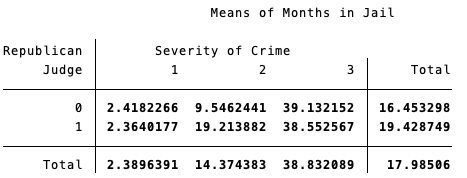
\includegraphics[width=90mm]{averages.png}
    \center
\end{figure}


\section{Compliers}
In the dataset, compliers would be defendants who receive shorter sentences from Democrat judges and receive longer sentences from Republican judges, holding severity of crime constant.

\section{Cycle of Crime Hypothesis}
For compliers, the cycle of crime hypothesis does seem to be true. For those who receive an additional month in jail, their likelihood of recidivism increases by 0.0443 points, which is significant at p \textless 0.001.

\end{document}
